\chapter{Návrh}\label{nuxe1vrh}

\section{Průběh výuky}\label{prux16fbux11bh-vuxfduky-2}

Před konkrétním návrhem přesného scénáře výuky se v této kapitole budu
nejdříve zabývat hrubým a obecnějším návrhem průběhu celé výuky.
Samotnou výuku rozdělím do tzv. momentů, které si i označím
identifikátory, pro možnost pozdější reference v textu. Výsledný průběh
pak dále zpracuji ve formě storyboards.

Celá výuka bude v češtině, jelikož se prozatím počítá pouze s nasazením
v české herně. Do herny však chodí i zahraniční návštěvníci. Rámec této
závěrečné práce nebude zahrnovat překlad do jiného jazyka, ovšem
aplikace bude na lokalizaci připravena.

\section{Momenty výuky}\label{momenty-vuxfduky}

Seznam klíčových momentů průběhu výuky v chronologickém pořadí:

\begin{itemize}
\tightlist
\item
  \textbf{M1} -- Uživatel je uvítán do herny, kterou navštívil.
\item
  \textbf{M2} -- Uživateli je vysvětleno, jaký bude průběh výuky.
\item
  \textbf{M3} -- Uživateli je umožněno výuku přeskočit.
\item
  \textbf{M4} -- Uživateli je představena play area a chaperone bounds.
\item
  \textbf{M5} -- Uživateli jsou představeny ovladače.
\item
  \textbf{M6} -- Uživateli je představeno každé tlačítko na ovladači a
  je požádán aby je stiskl.
\item
  \textbf{M7} -- Uživateli je vysvětleno, k čemu je určen spouštěč,
  který je mu zobrazen po skončení výuky.
\end{itemize}

\subsection{M1 Uvítání herny}\label{m1-uvuxedtuxe1nuxed-herny}

Jako první moment je herně posktynut velmi krátký prostor na její
prezentaci. Návštěvník je uvítán jménem herny do virtuální
reality. Zároveň je mu na krátký moment zobrazeno logo herny. Díky
tomuto prvku je aplikace blíže svázána s hernou a jedná se tak i o
jistou formu brandingu.

Díky tomuto prvku mohou mít o aplikaci zájem i jiné firmy provozující
herny virtuální reality, jelikož prozatím neexistuje žádná dostupná
aplikace pro virtuální realitu, která by nějakým způsobem prezentovala
hernu, kterou uživatel právě navštívil.

\subsection{M2 Vysvětlení průběhu
výuky}\label{m2-vysvux11btlenuxed-prux16fbux11bhu-vuxfduky}

Aby byl uživatel připravený a věděl, co jej čeká, je mu velmi stručně
přiblížen průběh výuky. Zároveň se tak může lépe v následujícím momentu
rozhodnout, zda bude výuku přeskakovat.

\subsection{M3 Možnost přeskočení
výuky}\label{m3-moux17enost-pux159eskoux10denuxed-vuxfduky}

Protože někteří uživatelé jsou již systému HTC Vive znalí, je jim
umožněno takovou výuku přeskočit a jsou rovnou přesunuti do části se
spouštěčem.

Přeskočení výuky lze provést stisknutím kombinace tlačítek na ovladači.
Na obou ovladačích bude uživatel nucen stisknout tlačítko spouště a
tlačítko nabídky. Tato kombinace bude uživateli představena a jde o
takovou kombinaci tlačítek, kterou neznalý uživatel omylem nestiskne.

Stisknutí těchto dvou tlačítek není úplně přirozené. Při běžném držení
má uživatel palec spíše v oblasti nad dotykovou plochou, nebo mírně pod
ní. Tlačítko nabídky se nachází nad dotykovou plochou. Zároveň stisknutí
obou tlačítek zároveň je mírně nepřirozené (je nepravděpodobné, že by
tato dvě tlačítka uživatel stiskl omylem, např. nevhodným úchopem
ovladače), ale zároveň ne nemožné, či obtížné.

\subsection{M4 Představení Play area a Chaperone
Bounds}\label{m4-pux159edstavenuxed-play-area-a-chaperone-bounds}

Jelikož bezpečnost uživatele a majetku herny je prioritní, jsou mu nejdříve
vysvětleny pravidla pohybu v prostoru.

Uživateli se na podlaze zobrazí ohraničení odpovídající velikosti a
pozici nastavené \emph{play area}. Je mu vysvětleno, k čemu \emph{play
area} slouží. Následně jsou mu představeny \emph{chaperone bounds}.
Uživatel je požádán, aby k hranici přistoupil, aby si funkcionalitu
vyzkoušel.

\begin{figure}
\centering
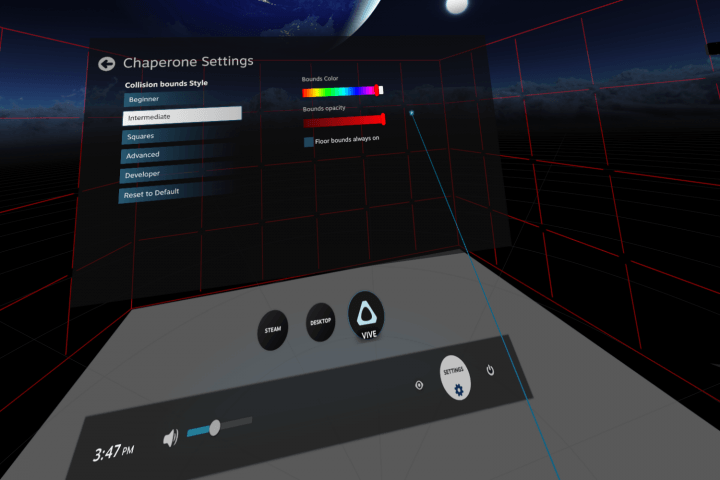
\includegraphics[width=12cm]{src/assets/chaperone.png}
\caption{Chaperone bounds a jejich možnosti v nastavení OpenVR}
\end{figure}

Tento přístup je tak inspirován výukou v aplikaci \emph{SteamVR
Tutorial}. Je však zkrácena o jedno opakování, aby tato část nebyla
příliš dlouhá. Ač bylo výše poznamenáno, že je žádoucí, aby byl na tuto
část kladen důraz, je předpokládáno, že jedno přistoupení k mřížce uživateli
stačí k tomu, aby funkci pochopil a na zobrazení mřížky v budoucnu
reagoval.

\subsection{M5 Představení
ovladače}\label{m5-pux159edstavenuxed-ovladaux10de}

Uživatel je požádán, aby si prohlédl ohraničení místnosti a ve chvíli,
kdy bude připraven pokračovat ve výuce dále, si stoupl do středu
místnosti a zvedl své ovladače před sebe tak, aby na ně viděl.

V aplikaci bude vykreslován velmi přesný model ovladače, takže uživatel
může pohodlně prozkoumat, jak ovladač vypadá, pokusit se nalézt všechna
tlačítka sám a najít správný úchop pro vlastní komfort.

Skriptově nebude podmíněno, aby si uživatel stoupl do středu místnosti.
Instrukce slouží spíše k úpravě pozice uživatele. Poslední jeho poloha
je totiž u kraje místnosti, kde právě před chvílí zkoumal Chaperone
bounds. Ač mají Chaperone bounds od reálně vyměřené velikosti místnosti
určitý odstup, stále se může stát, že uživatel ve chvíli, kdy je
požádán, aby zvedl natažené ruce před sebe, natáhne ruce příliš a může
ovladačem uhodit do stěny, která je před ním.

\subsection{M6 Představení
tlačítek}\label{m6-pux159edstavenuxed-tlaux10duxedtek}

Každé tlačítko je uživateli postupně představeno, zvýrazněno zobrazením
titulku názvu tlačítka a je požádán, aby tlačítko stiskl, nebo s ním
provedl nějakou interakci, a to v následujícím pořadí:

\begin{itemize}
\tightlist
\item
  Tlačítko spouště
\item
  Boční tlačítka
\item
  Dotyková plocha
\item
  Tlačítko nabídky a systémové tlačítko
\end{itemize}

Po každém požádání o stisk tlačítka je uživatel jen přibližně seznámen s
tím, k čemu se tlačítko běžně používá. Je však nutné u návrhu scénáře
dát pozor, aby takové informace nebyly zavádějící, protože jak bylo již
v analýze zmíněno, tlačítka si aplikace mapují podle vlastního uvážení
a každá aplikace tak tlačítka používá k různým činnostem.

\begin{figure}
\centering
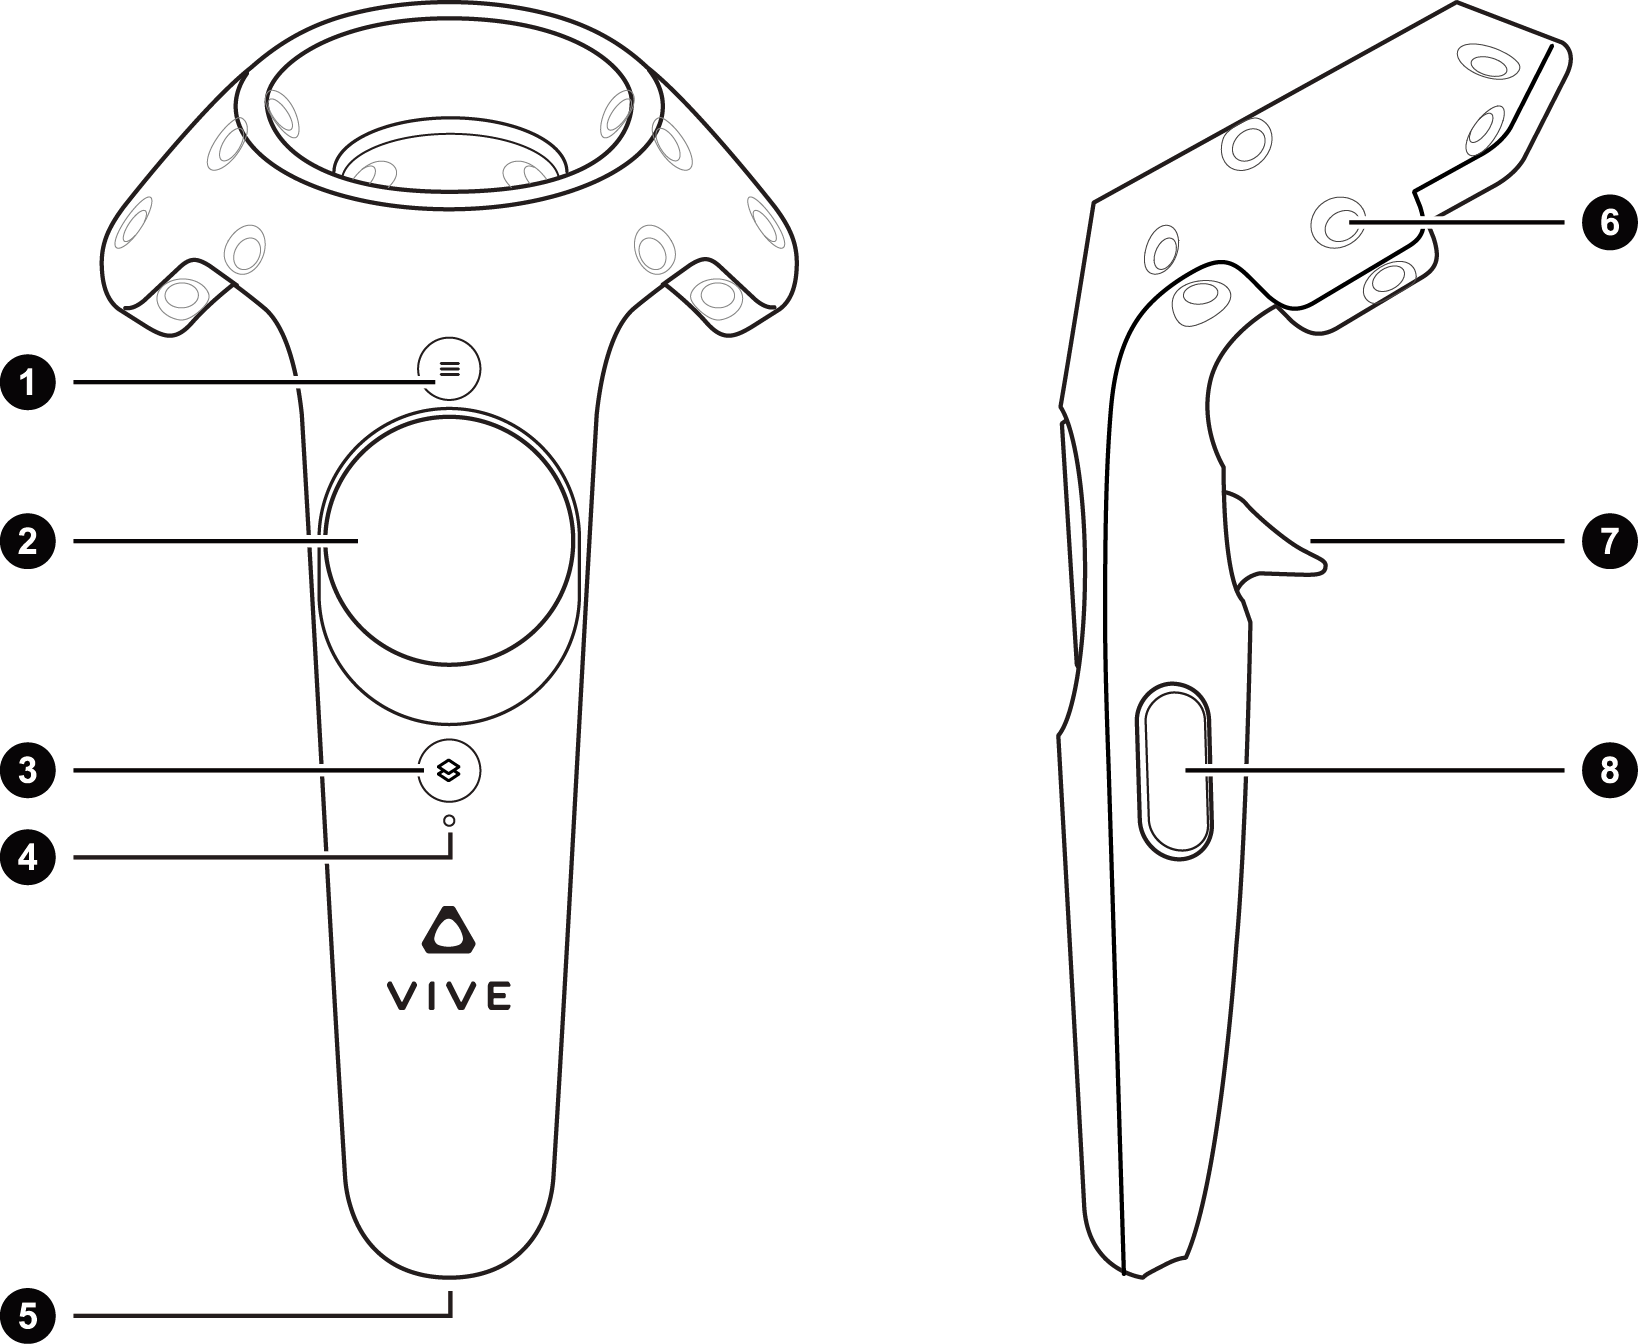
\includegraphics[width=10cm]{src/assets/vive-controller.png}
\caption{Náčrt ovladače HTC Vive\autocite{htcvivemanual}}
\end{figure}

Protože je tlačítko spouště důležité, je do výuky přidán prvek
laserového ukazovátka, pomocí kterého se uživatel naučí s ovladačem
mířit a spouští vybírat. Mělo by to tak podvědomě utvrdit často VR
aplikacemi využívaný koncept navigace v nabídkách -- ukázáním a výběrem
spouští.

Následně je uživatel požádán, aby tlačítko spouště stiskl, což vyvolá
akci ve formě zesílení laserového paprsku a efektu na konci paprsku.
Uživatel je požádán, aby namířil na terč, který bude pro účely tohoto
kroku do scény umístěn a stiskl spoušť. Je tak v rychlosti uveden do
schopnosti mířit ovladačem.

Protože laserový paprsek vypaluje do okolí stopy, uživatel může být
podvědomě podnícen práci se spouští procvičit více a to tak, že začne do
okolí vypalovat další stopy. Ač je hned následně pobídnut, aby stiskl
boční tlačítko, může tak stále činit a dále používat tlačítko spouště s
laserovým paprskem.

Poté, co uživatel stikne boční tlačítko, je mu představena dotyková
plocha. Je důležité, aby uživatel pochopil, že má dvě funkce. Pohyb
prstem přes plochu a její stisknutí. Na ovladači přes dotykovou plochu
se zobrazí barevný kruh a uživatel je požádán, aby přes plochu přejížděl
prstem, vybral si barvu a dotykovou plochu stiskl. Výběrem barvy a
stikem dotykového tlačítka je uživateli změněna barva laserového
ukazovátka. Opět jej to může podpořit v další spontánní činnosti s
ovladači.

Jako poslední jsou mu představena tlačítka nabídky a systémové tlačítko.
Tady uživatel výjimečně není požádán o stisk těchto tlačítek, jelikož
systémové tlačítko otevírá \emph{SteamVR Dashboard}, který záměrně
uživateli představit nechceme. V rámci urychlení pak nechceme uživatele
žádat o stisk tlačítka nabídky.

Funkce obou tlačítek je však vysvětlena a nedochází ve výuce ke snaze
přesvědčit jej, aby systémové tlačítko nepoužíval. Místo toho je mu
vysvětleno, k čemu slouží, co se po stisku stane a velmi mírně s dobrou
volbou slov doporučíme procházení \emph{SteamVR Dashboard} pouze
zkušenějším uživatelům. Chceme však toto tlačítko vysvětlit i uživatelům
neznalým, aby při stisku tohoto tlačítka nezpanikařili a vzpomněli si,
která je naučila stisk tohoto tlačítka v případě, že nějakou systémovou
nabídku otevřeli omylem.

\subsection{M7 Představení
spouštěče}\label{m7-pux159edstavenuxed-spouux161tux11bux10de}

Po skončení výuky je uživateli oznámeno, že mu bylo sděleno vše, co o
systému pro tuto chvíli potřebuje vědět a je mu vysvětleno, co se bude
dále dít.

Krátce je mu představeno, co před sebou vidí, k čemu je spouštěč určen a
jak může spustit svůj první VR zážitek.

\section{Návrh výuky}\label{nuxe1vrh-vuxfduky}

Poté, co byl specifikován hrubý návrh scénáře výuky a její momenty, lze
z těchto momentů sestavit konkrétní podobu výuky.

\subsection{Návrh scénáře}\label{nuxe1vrh-scuxe9nuxe1ux159e}

První část návrhu výuky je sestavení scénáře, který pak lze velmi
efektivně využít pro skriptování průběhu, zobrazení přepisu a k dabování
mluveného slova.

Ve scénáři jsou uvedeny identifikátory momentů. Označují části, které
vycházejí ze momentů zadefinovaných výše.

Tento konkrétní přepis scénáře je lokalizován do češtiny a je určen pro
použití v české herně \emph{Virtualnirealita.cz}, kde bude později
produkčně nasazen. Aplikaci bude však možné připravit i pro jiné herny,
nebo jiná prostředí. Bude však nutné pozměnit tento scénář, konkrétně v
místech úvodu a závěru. Vše bude možné v aplikaci upravit bez nutnosti
zásahu do kódu.

\begin{center}\rule{0.5\linewidth}{\linethickness}\end{center}

\emph{Zobrazí se logo herny. {[}M1{]}}

\textbf{Průvodce:} Vítejte v herně Virtualnirealita.cz! Tato krátká
výuka vás provede vstupem do virtuální reality. \emph{{[}M2{]}}

\emph{Zobrazí se instrukce pro přeskočení výuky na obrazovce.}

\textbf{Průvodce:} Pokud s virtuální realitou již máte zkušenosti a
výuku chcete přeskočit, stiskněte kombinaci tlačítek menu a spouště.
\emph{{[}M3{]}}

\emph{- krátká pauza -}

\textbf{Průvodce:} Rozhlédněte se kolem sebe a na podlahu. Ohraničení,
které můžete vidět na zemi je místo, ve kterém se lze volně pohybovat v
průběhu vašich zážitků ve virtuální realitě. \emph{{[}M4{]}}

\textbf{Průvodce:} Toto ohraničení však není vidět vždy, proto se
zobrazuje pomocná mřížka, která vás na tyto hranice upozorní, pokud se
je pokusíte překročit.

\textbf{Průvodce:} Nyní se zkuste pomalu k hranici přiblížit, abyste si
vyzkoušeli, jak to funguje. Za tuto hranici dále nechoďte.

\emph{- krátká pauza -}

\textbf{Průvodce:} Až dokončíte prozkoumávání ohraničení, vraťte se
doprostřed místnosti a zvedněte obě ruce před sebe. Řekneme si něco k
ovladačům, které máte v ruce. \emph{{[}M5{]}}

\emph{Čekání na reakci uživatele: zvednutí rukou před sebe\ldots{}}

\textbf{Průvodce:} Toto jsou ovladače systému HTC Vive. Nyní vám
představíme tlačítka těchto ovladačů. \emph{{[}M6{]}}

\emph{Zvýrazní se tlačítko spouště.}

\textbf{Průvodce:} Toto je tlačítko spouště. Slouží ve hrách většinou
jako tlačítko pro výstřel, nebo výběr položky v menu.

\emph{Uživateli začne z pravého ovladače vyzařovat slabý laserový
paprsek.}

\textbf{Průvodce:} Namiřte laserové ukazovátko na terč a stiskněte
spoušť.

\emph{Čekání na reakci uživatele: namíření na terč a stisk
spouště\ldots{}}

\emph{Zvýrazní se boční tlačítko.}

\textbf{Průvodce:} Perfektní! Toto je boční tlačítko, které lze
stisknout z libovolné strany. Slouží jako alternativní funkce, například
pro přebíjení zbraně. Stiskněte jej.

\emph{Čekání na reakci uživatele: stisk bočního tlačítka\ldots{}}

\emph{Zvýrazní se dotyková plocha.}

\textbf{Průvodce:} Dobře. Toto je dotyková část ovladače. Můžete po ní
přejíždět prstem a také ji stisknout. Přejížděním prstu vyberte barvu a
stisknutím dotykové plochy vyberte barvu svého laserového ukazovátka.

\emph{Čekání na reakci uživatele: stisk dotykové plochy\ldots{}}

\textbf{Průvodce:} Skvěle! Zbývají nám dvě tlačítka. Menu tlačítko a
systémové tlačítko.

\emph{Zvýrazní se menu tlačítko.}

\textbf{Průvodce:} Menu tlačítko slouží většinou k vyvolání nabídky ve
hře. Často můžete tímto tlačítkem také pozastavit hru.

\emph{Zvýrazní se systémové tlačítko.}

\textbf{Průvodce:} Systémové tlačítko pak otevírá rozhraní systému
Steam. Pokud jste s platformou Steam seznámeni, můžete toto tlačítko
používat pro procházení knihovnou. Stejným tlačítkem toto rozhraní i
můžete zavřít.

\textbf{Průvodce:} Nyní jste připraveni spustit svůj první zážitek ve
virtuální realitě. Před sebou vidíte knihovnu dostupných aplikací naší
herny. Vyberte si, o který zážitek máte zájem, namiřte na něj a
stiskněte spoušť. \emph{{[}M7{]}}

\begin{center}\rule{0.5\linewidth}{\linethickness}\end{center}

\subsection{Storyboards}\label{storyboards}

Pro lepší vizualizaci je k podrobnému konkrétnímu scénáři i ilustrován
průběh výuky ve formě storyboards.

\begin{quote}
TODO: Přidat obrázek storyboards.
\end{quote}

\section{Návrh spouštěče}\label{nuxe1vrh-spouux161tux11bux10de}

Spouštěč je funkcionalita aplikace navazující po výuce. Je určen k tomu,
aby nahradil stávající řešení výběru VR aplikací skrze \emph{SteamVR
Dashboard}, které se ukázalo být nevhodné pro použití v prostředí herny.

Podle funkčních požadavků a v kontrastu s existujícími řešení v podobě
\emph{SteamVR Dashboard} a \emph{Oculus Home} chceme vytvořit takový
spouštěč, který bude pro uživatele jednoduchý, bude brát v potaz fakt,
že uživatel může být v systému virtuální reality stále nováček a nemusí
znát tituly podle jejich názvu. 

Nechceme uživatele zatěžovat v herně
nerelevantními komunitními funkcemi. Tato funkce by měla nahradit
povinnost obsluhy dotazovat se návštěvníků, co mají rádi a odhadovat, o
jaký typ zážitku by mohli mít zájem.

\subsection{Návrh rozhraní}\label{nuxe1vrh-rozhranuxed}

Pro rozhraní lze využít celý prostor kolem uživatele. Nebude se jednat o
typ rozhraní, které můžeme vidět u \emph{SteamVR Dashboard} (ploché
dvourozměrné rozhraní vykreslované na malou plochu před uživatelem).
Základní myšlenka rozhraní je přístup k výběru VR aplikací skrz hlavní
primární obrazovku spouštěče. Oba zkoumané existující řešení, která byla
zmíněna výše, mají výběr VR aplikací ukrytý pod tlačíkem ``Library'',
což dělá rozhraní složitější.

Jako první bude uvádět rozhraní velký nadpis vyzývající uživatele k
činnosti: ``Vyberte si VR aplikaci''. Pod ním bude zobrazen název
aktuálně otevřené kategorie s šipkou evokující možnost výběru, kterou
může uživatel provést změnu aktuálně zobrazené kategorie. Pod výběřem
kategorií se nachází mřížka s aplikacemi. Mřížka bude na výšku čtyři
řádky vysoká a na šířku bude obsahovat počet sloupců daný maximálním
počtem sloupců zobrazitelných v konkrétní místnosti.

\begin{figure}
\centering
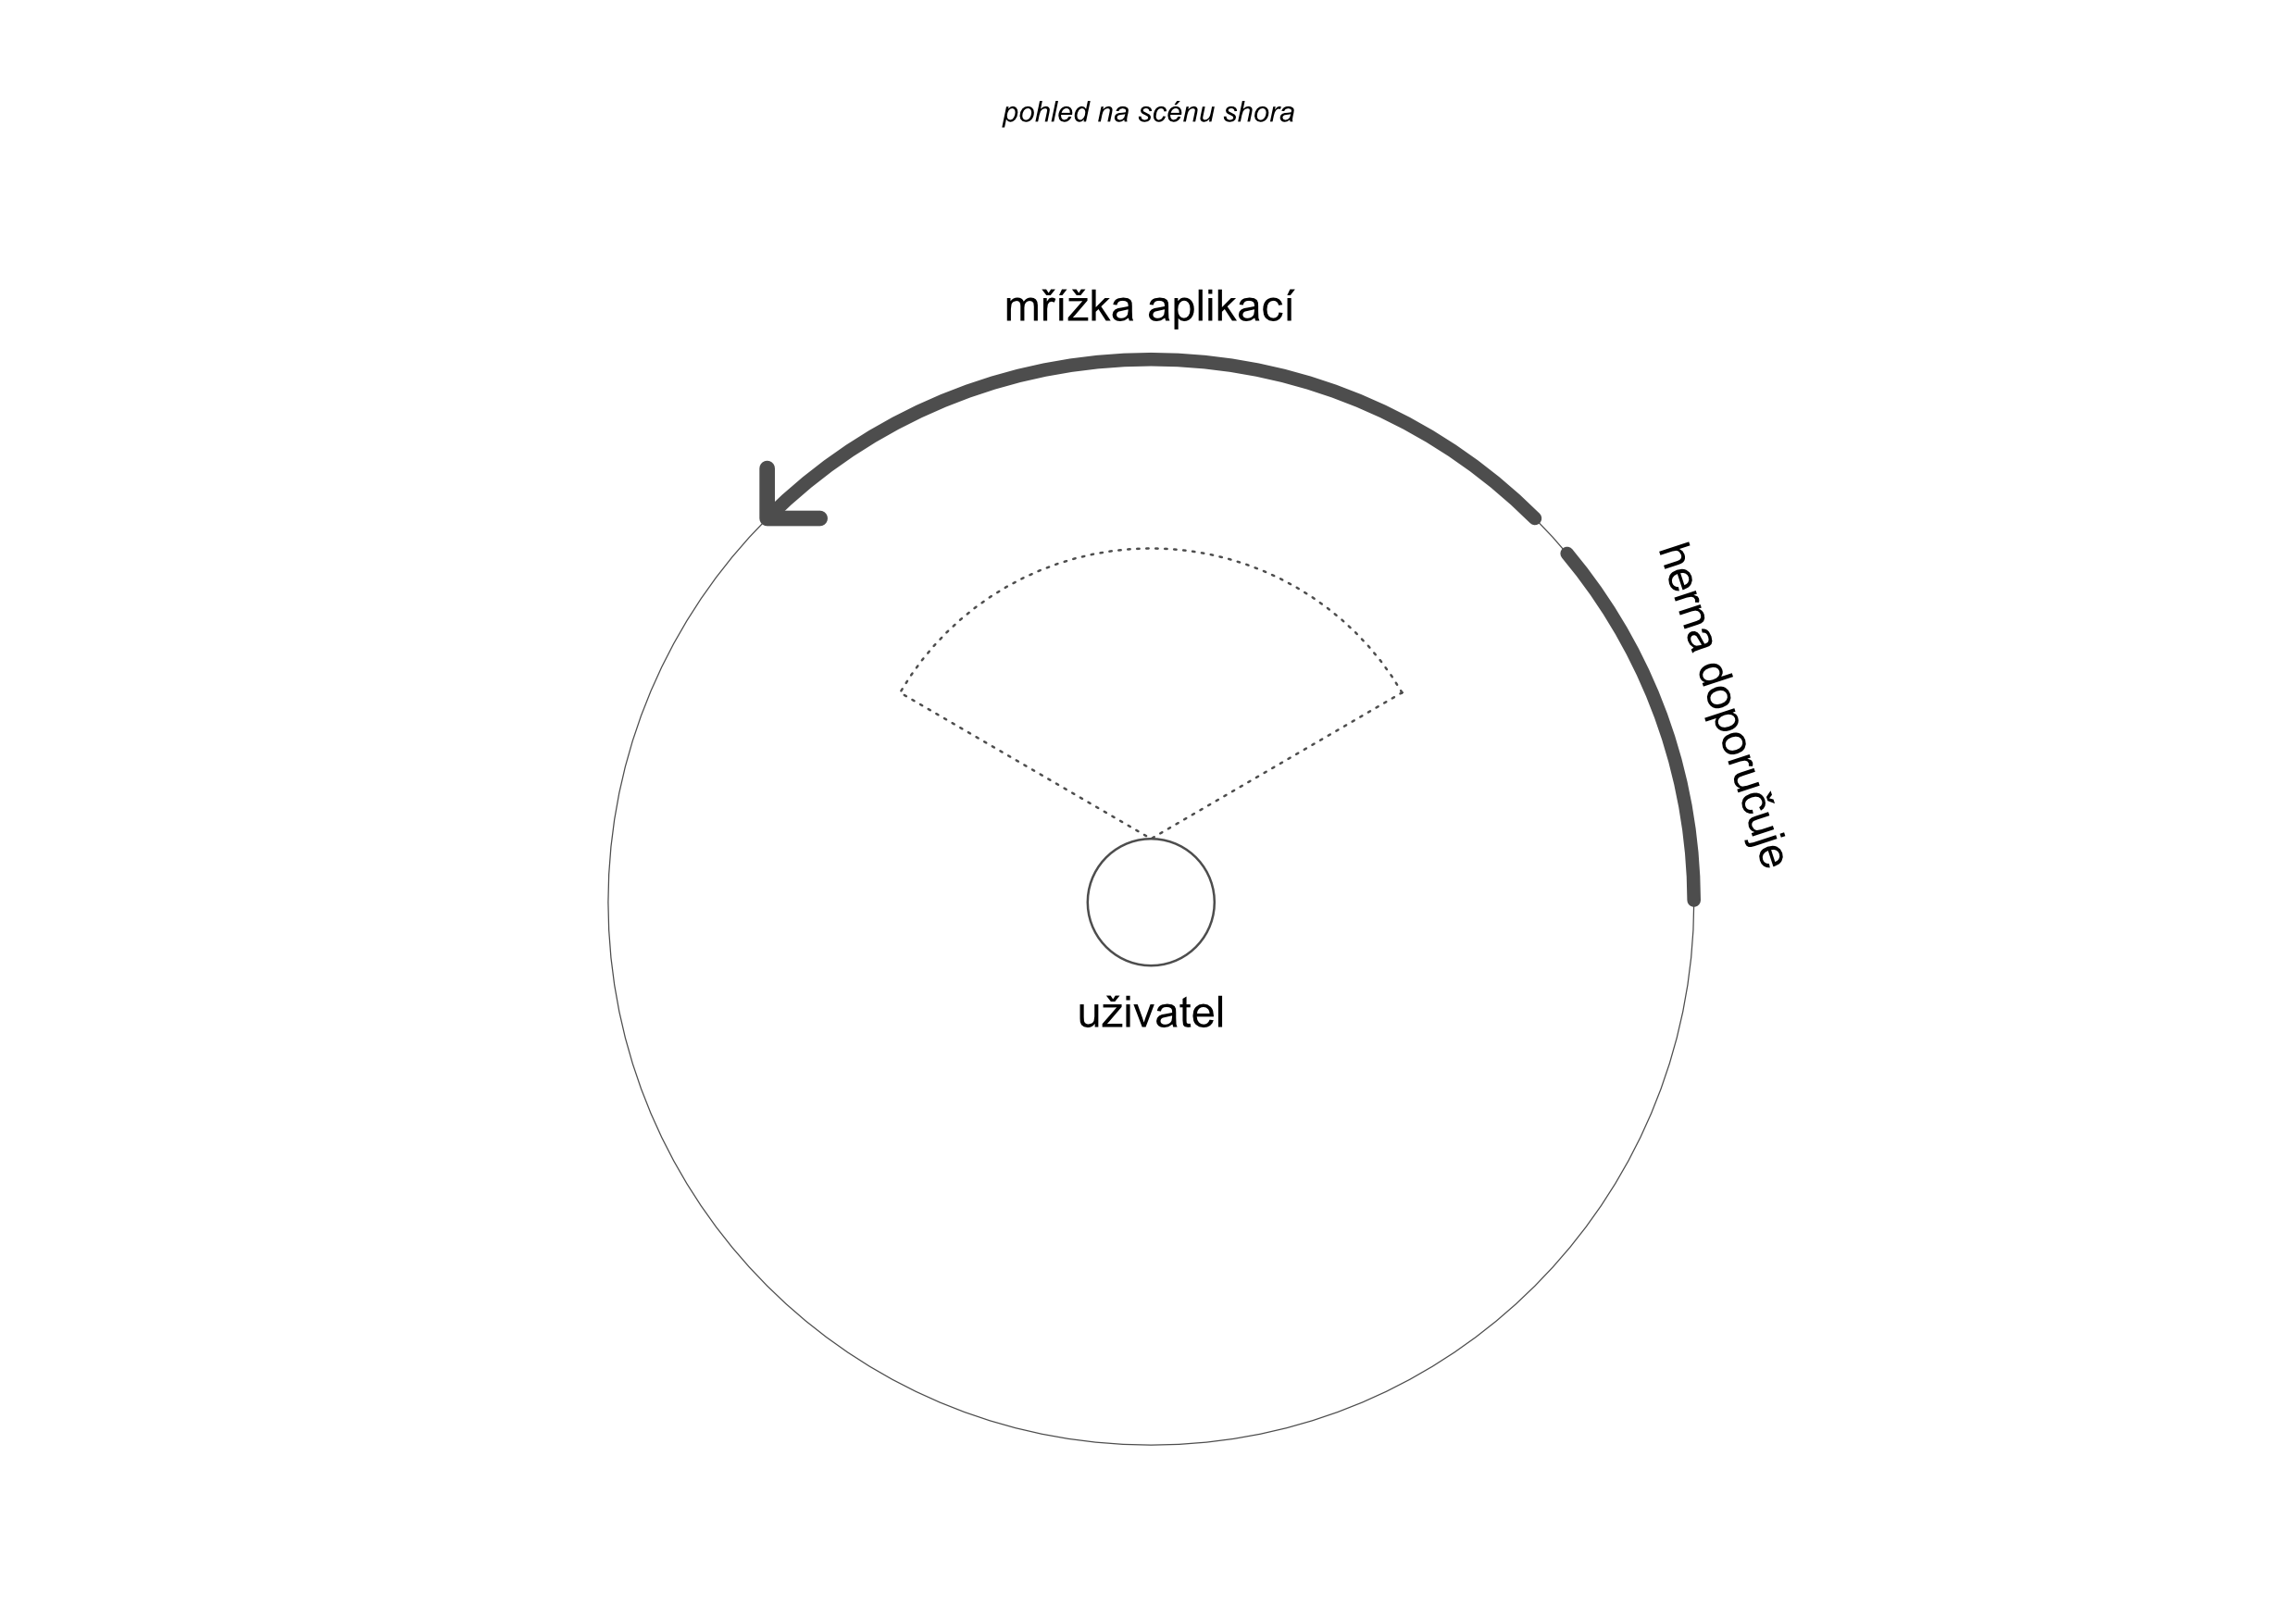
\includegraphics[width=\textwidth]{src/assets/wireframe-ui.png}
\caption{Rozložení prvků rozhraní kolem uživatele}
\end{figure}

VR aplikace budou v mřížce zobrazovány velmi podobně, jako jsou
zobrazovány v existujících spouštěčích -- vizuální obdélníkový banner s
vizuálem aplikace. Velký rozdíl se však projeví při výběru banneru.

Aplikace zobrazí po výběru svůj rychlý detail. Místo vizuálního banneru zaujme
krátké video pořízené z aplikace (tzv. in-game gameplay), které se bude
opakovat. Nepůjde tedy o vizuál autorů aplikace nebo trailer, ale o
realistický záznam přímo z aplikace. Uživatel bude schopen velmi přesně
odhadnout, o čem aplikace je, jaká je její vizuální úroveň a přibližně
odhadne i hratelnost a celkový dojem z aplikace, ještě dřív, než ji
spustí. Napravo od videa pak bude detail doplněn o celý název titulu,
krátkým popisem a kategorizací podle žánru a intenzity. 

Celý tento blok
detailu apliakce bude k uživateli mírně přiblížen a ostatní prvky budou
potlačeny do pozadí.

\begin{figure}
\centering
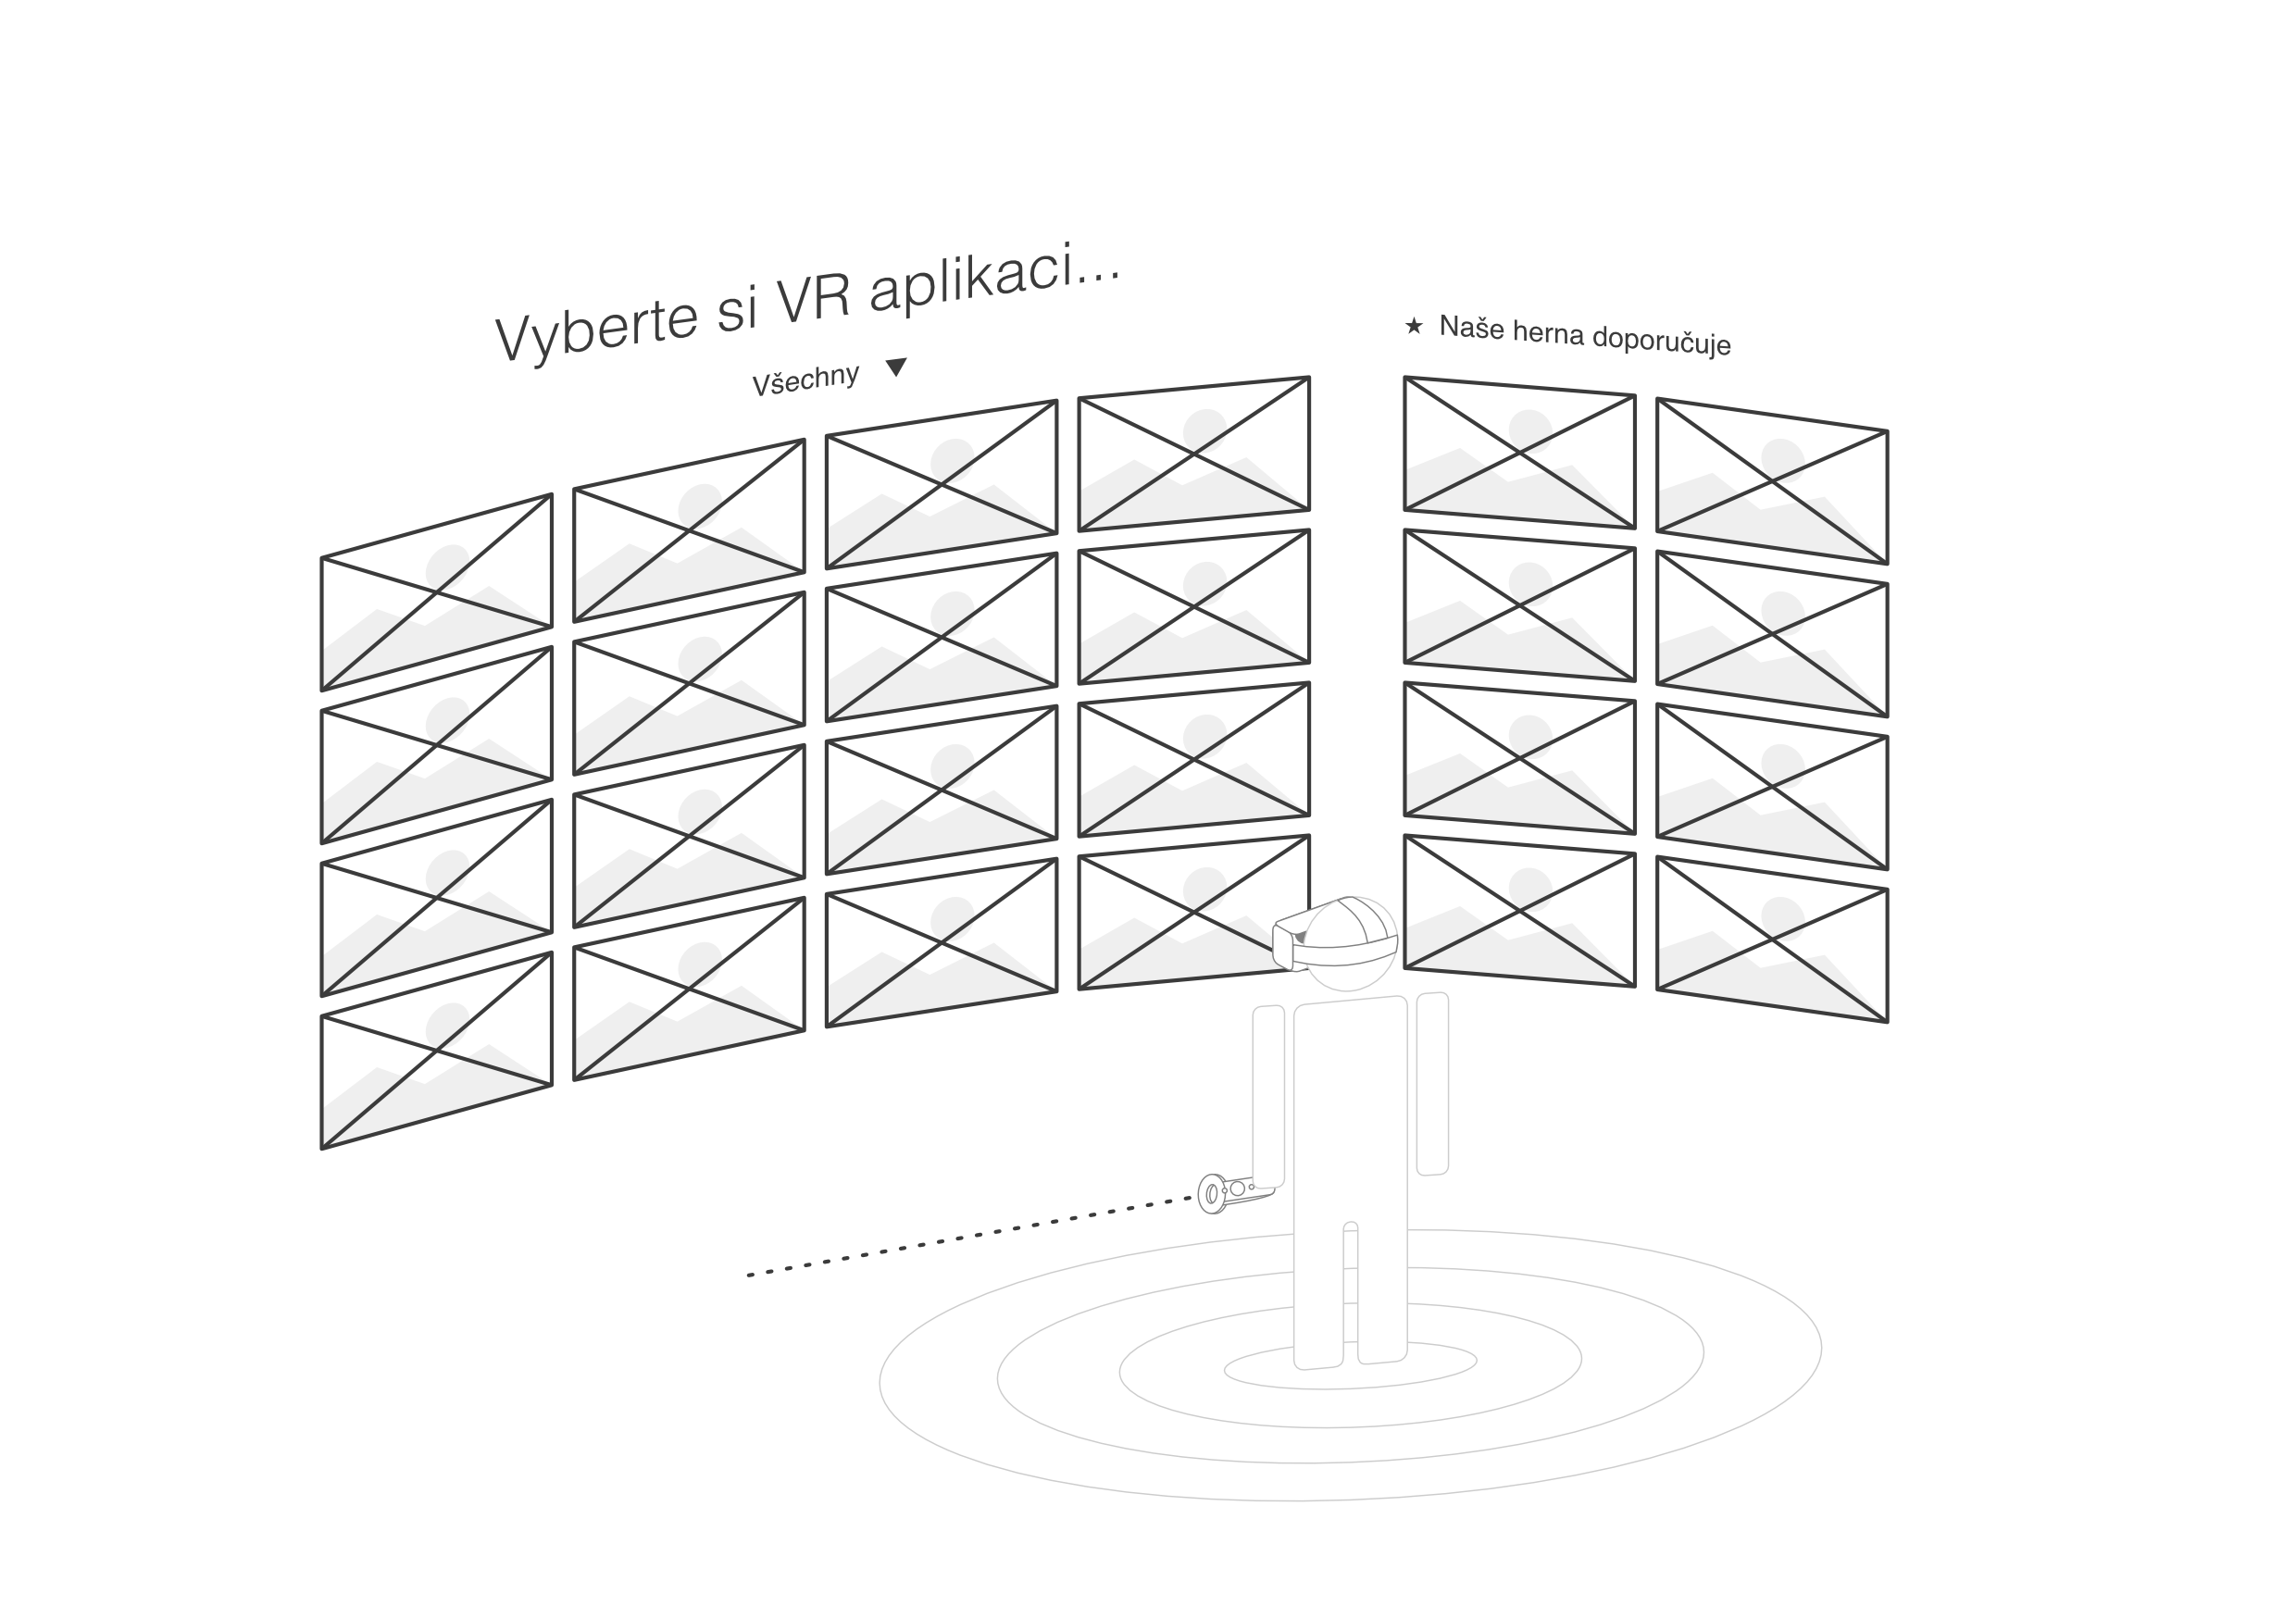
\includegraphics[width=\textwidth]{src/assets/wireframe-grid.png}
\caption{Základní stav aplikace spouštěče}
\end{figure}

Mřížka těchto bannerů se bude zobrazovat v kruhu okolo uživatele. Hlavní
mřížka aplikací bude zarovnána k pravému ``virtuálnímu okraji'', za
kterým budou dva sloupce dalších bannerů, označených jako ``Naše herna
doporučuje''. Tyto bannery bude volit herna jako doporučené aplikace pro
své zákazníky a bude obsahovat maximální počet 8 aplikací. 

Pravý ``virtuální okraj'' se bude nacházet po pravé ruce uživatele a hlavní
mřížka aplikace se bude podle počtu zobrazených aplikací rozšiřovat
proti směru hodinových ručiček o obvodu kruhu, na kterém se mřížka
zobrazuje. Pokud počet aplikací bude větší, než prostor k zobrazení
bannerů na mřížce, zobrazí se pod mřížkou přepínač stránek.

\begin{figure}
\centering
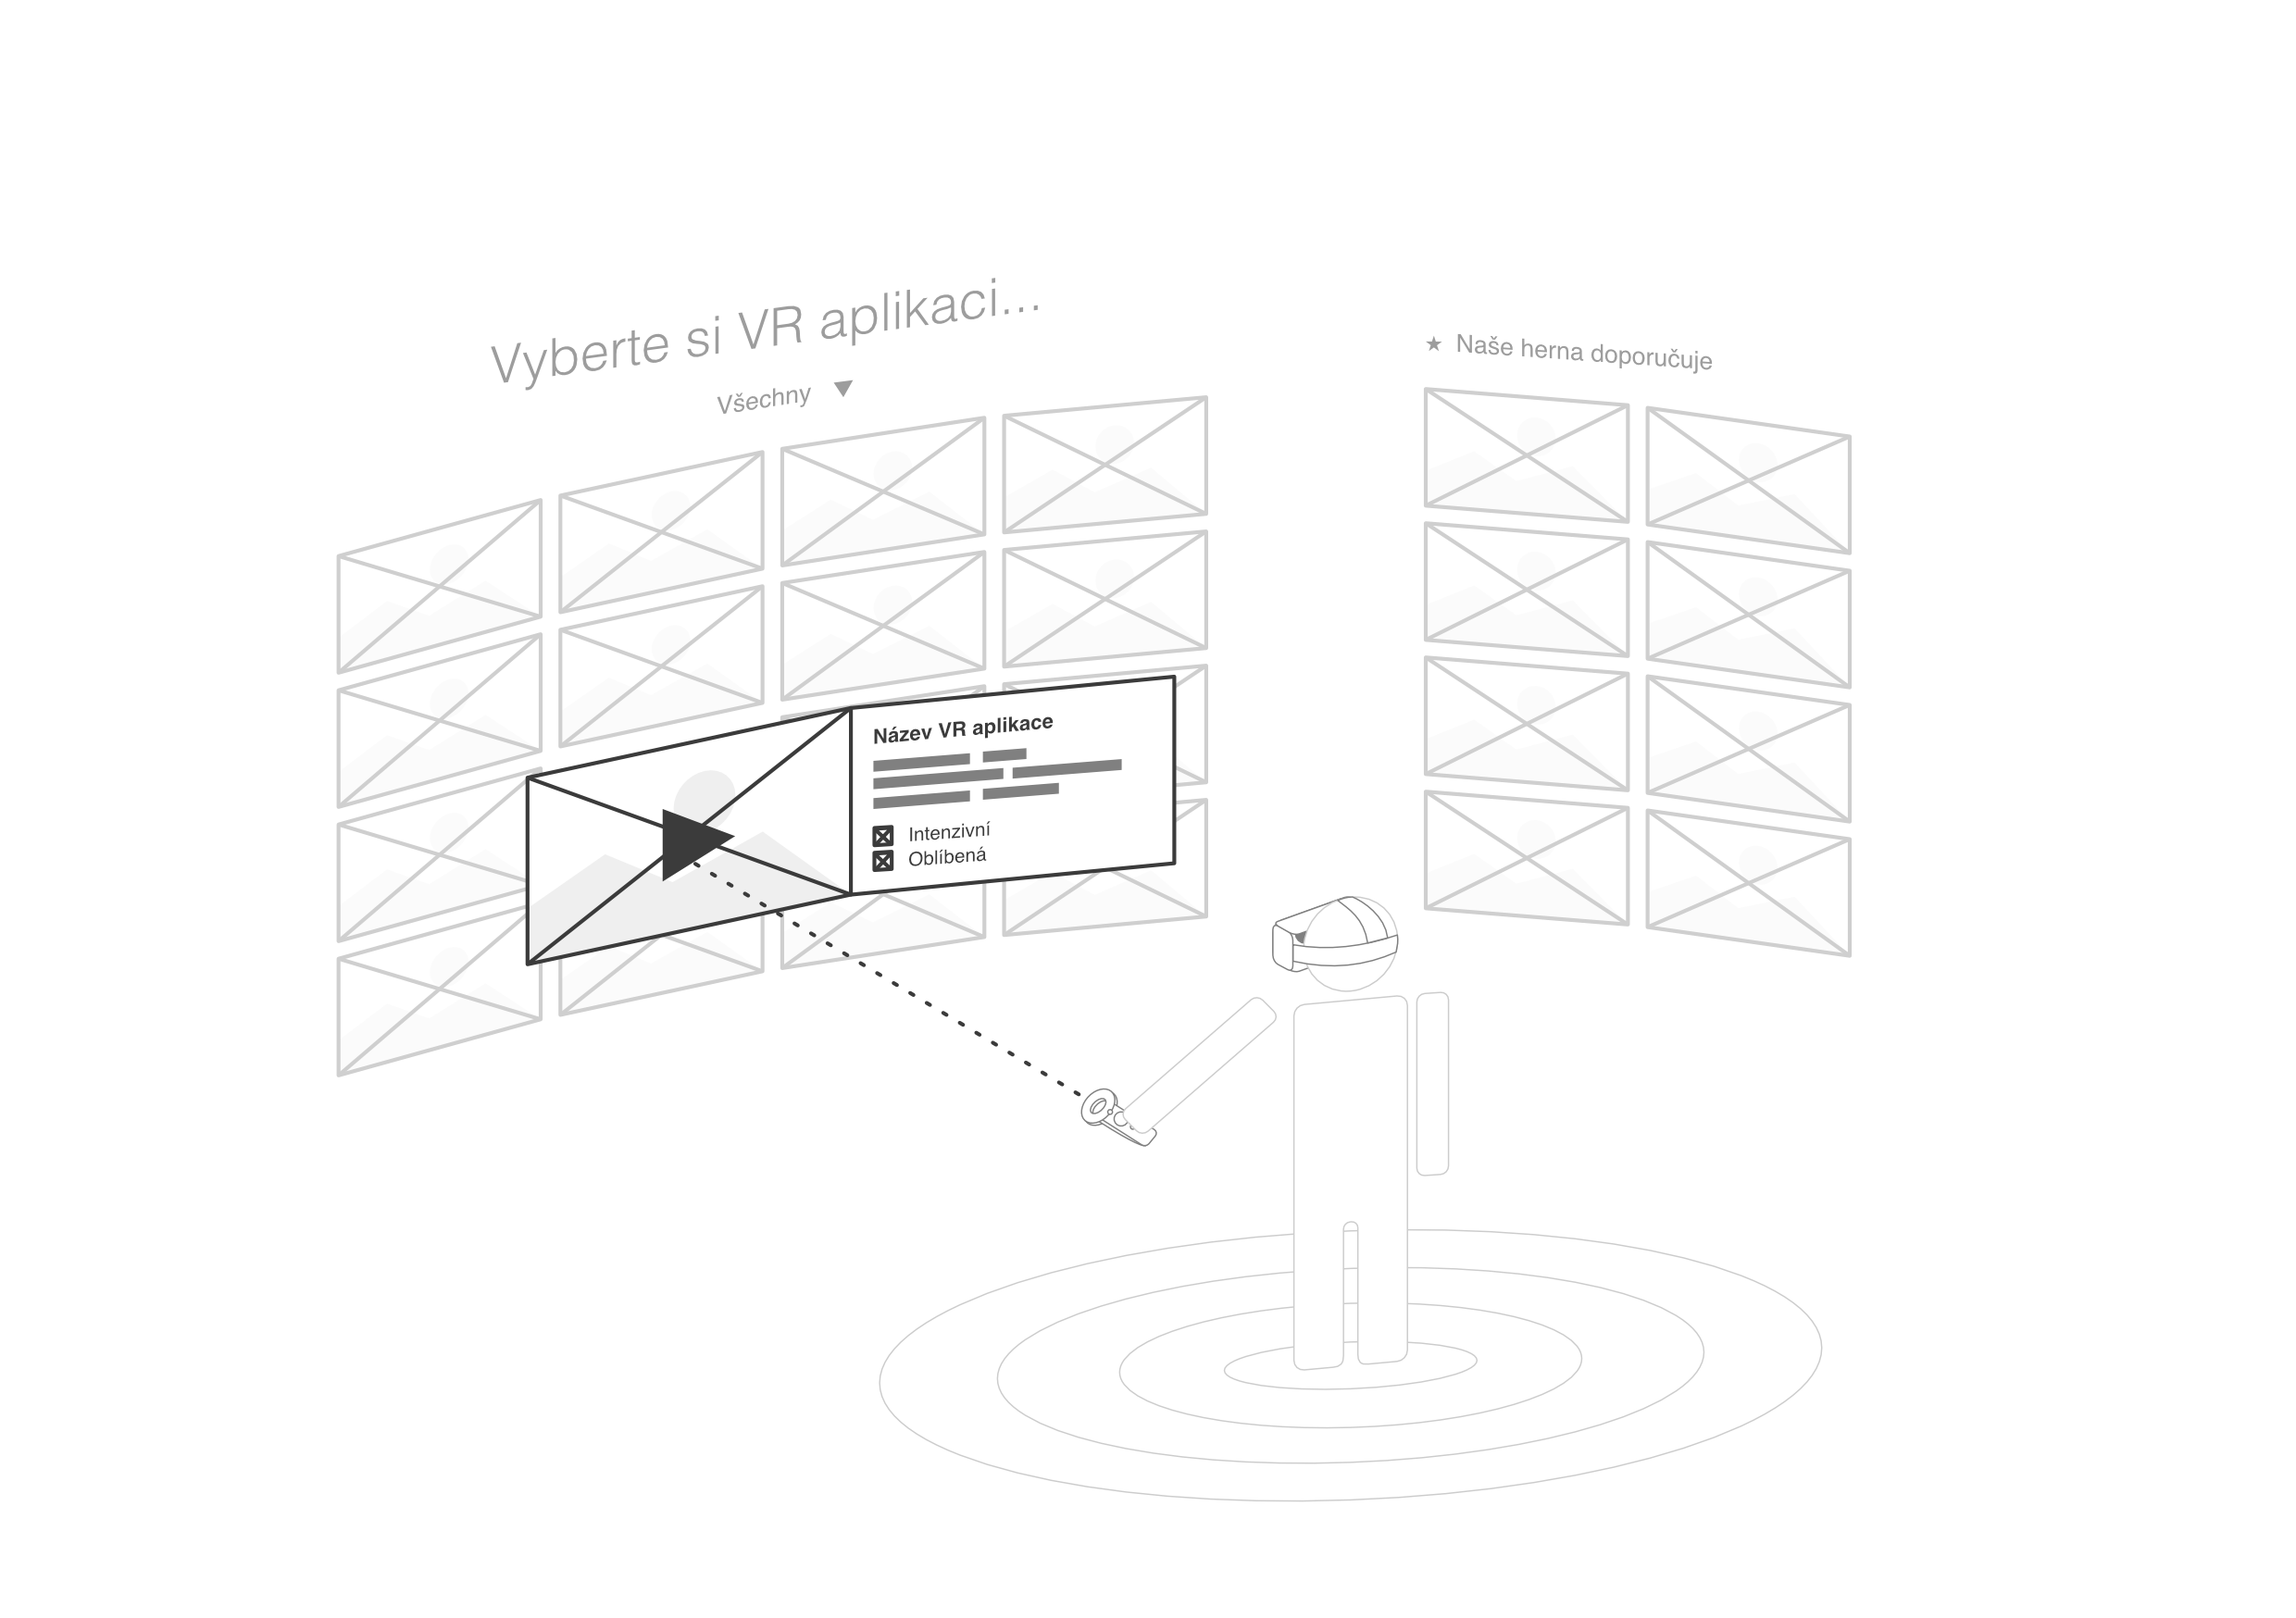
\includegraphics[width=\textwidth]{src/assets/wireframe-detail.png}
\caption{Detail aplikace po ukázání na jeho položku v mřížce}
\end{figure}

Po stisku tlatíčka pro změnu kategorie se potlačí pozadí stejným
způsobem, jako při práci s detailem aplikace. Do popředí se vyzobrazí
velmi jednoduchá nabídka v podobě seznamu dostupných kategorií, ze
kterých může uživatel vybírat. První oddělená položka této nabídky bude
tlačítko pro návrat nazvané ``Zpět''.

\begin{figure}
\centering
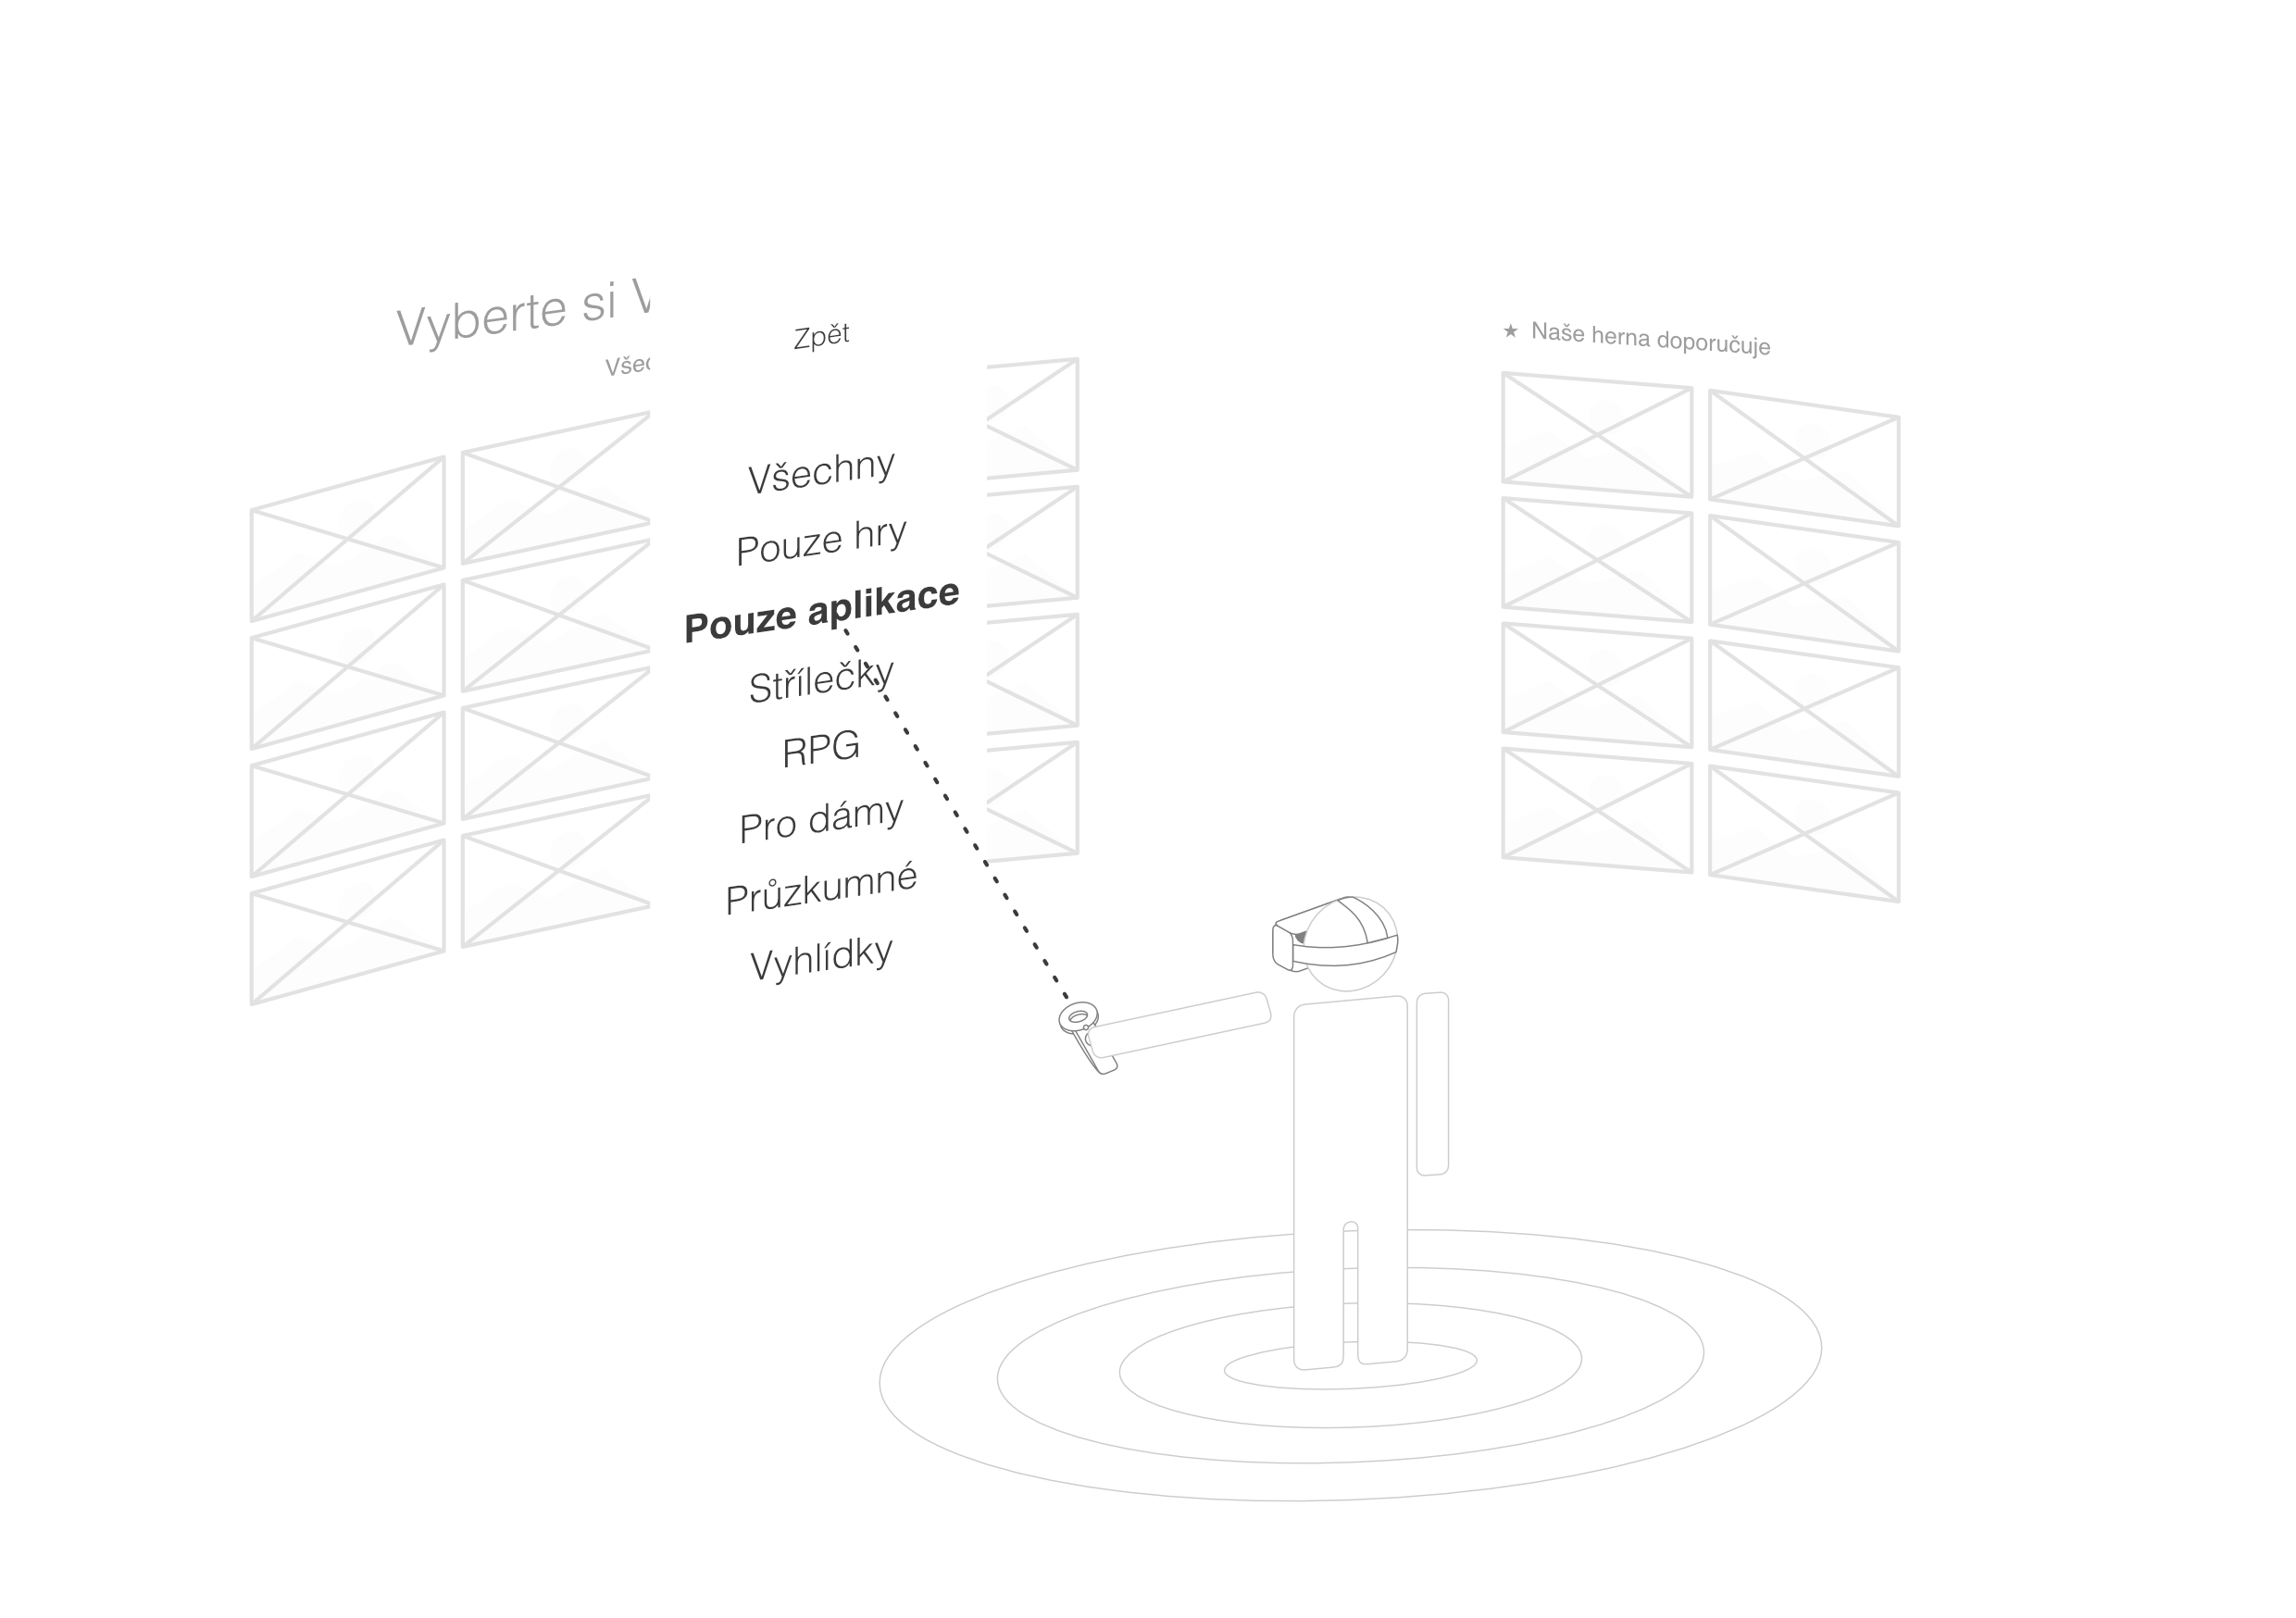
\includegraphics[width=\textwidth]{src/assets/wireframe-categ.png}
\caption{Výběr kategorie po kliknutí na prvek výběru kategorie}
\end{figure}

Rozhraní by tak mělo být velmi přehledné a především jednoduché.
Uživatel se v rozhraní nemá kde ztratit, rozhraní nemá přechod na jiné
obrazovky či stavy, s vyjímkou nabídky kategorií.
